\section{Abbildungsmaßstab des Kamerasystems}
Bevor das Plasma gezündet wird, muss der Abbildungsmaßstab der Messvorrichtung bestimmt werden. Hierzu vermessen wir den Abstand der unteren Elektrode zum Rand der Kammer bei verschiedenen Kamerapositionen und lassen uns mithilfe des Programmes \glqq uEyeCockpit\grqq{} die Länge dieser Distanz in Pixeln ausgeben. Damit erhalten wir:

\begin{table}[ht]
    \centering
    \begin{tabular}{c|c}
         Kameraabstand/Zoll& Distanz/Pixel \\\hline
         0.8 & 34 \\
         0.0 & 914 \\
    \end{tabular}
    \caption{Bestimmung des Abbildungsmaßstabes}
    \label{tab:abbmaß}
\end{table}

Der Abbildungsmaßstab A ergibt sich dann zu:
$$
    A=\frac{(0.8-0.0)Zoll*2,54*10^4\frac{cm}{Zoll}}{(914-34)Pixel}=23,09\frac{\mu m}{Pixel} 
$$

\section{Herstellung des Kristalls}
Nun leiten wir Argon-Gas in die Kammer; Dabei wird der Druck auf 40\,Pa gesetzt. Ab einer RF-Spannug von 1,15\,V zündet das Plasma. Die Spannung wird nun auf 0,15\,V reduziert, wobei der Plasmazstand des Gases erhalten bleibt. Anschließend werden die Plastikpartikel aus Melamin-Formaldehyd mit einem Dispenser in die Kammer gebracht. Die Partikel ordnen sich nach einer Zeit von 1-2\,min an und bleiben (in guter Näherung) in Position; Der Plasmakristall wurde hergestellt. An sämtlichen Rändern des Kristalls bewegen sich die Partikel recht stark, nur im inneren der Struktur sind die Teilchen fix. Im unteren Bereich des Kristalls haben sich die Plastikkügelchen \glqq geklumpt\grqq{} (große Punkte im Bild); Durch das erhöhte Gewicht werden sie nach unten gezogen (siehe Abbildung \ref{fig:groWo}).


\begin{figure}[ht]
    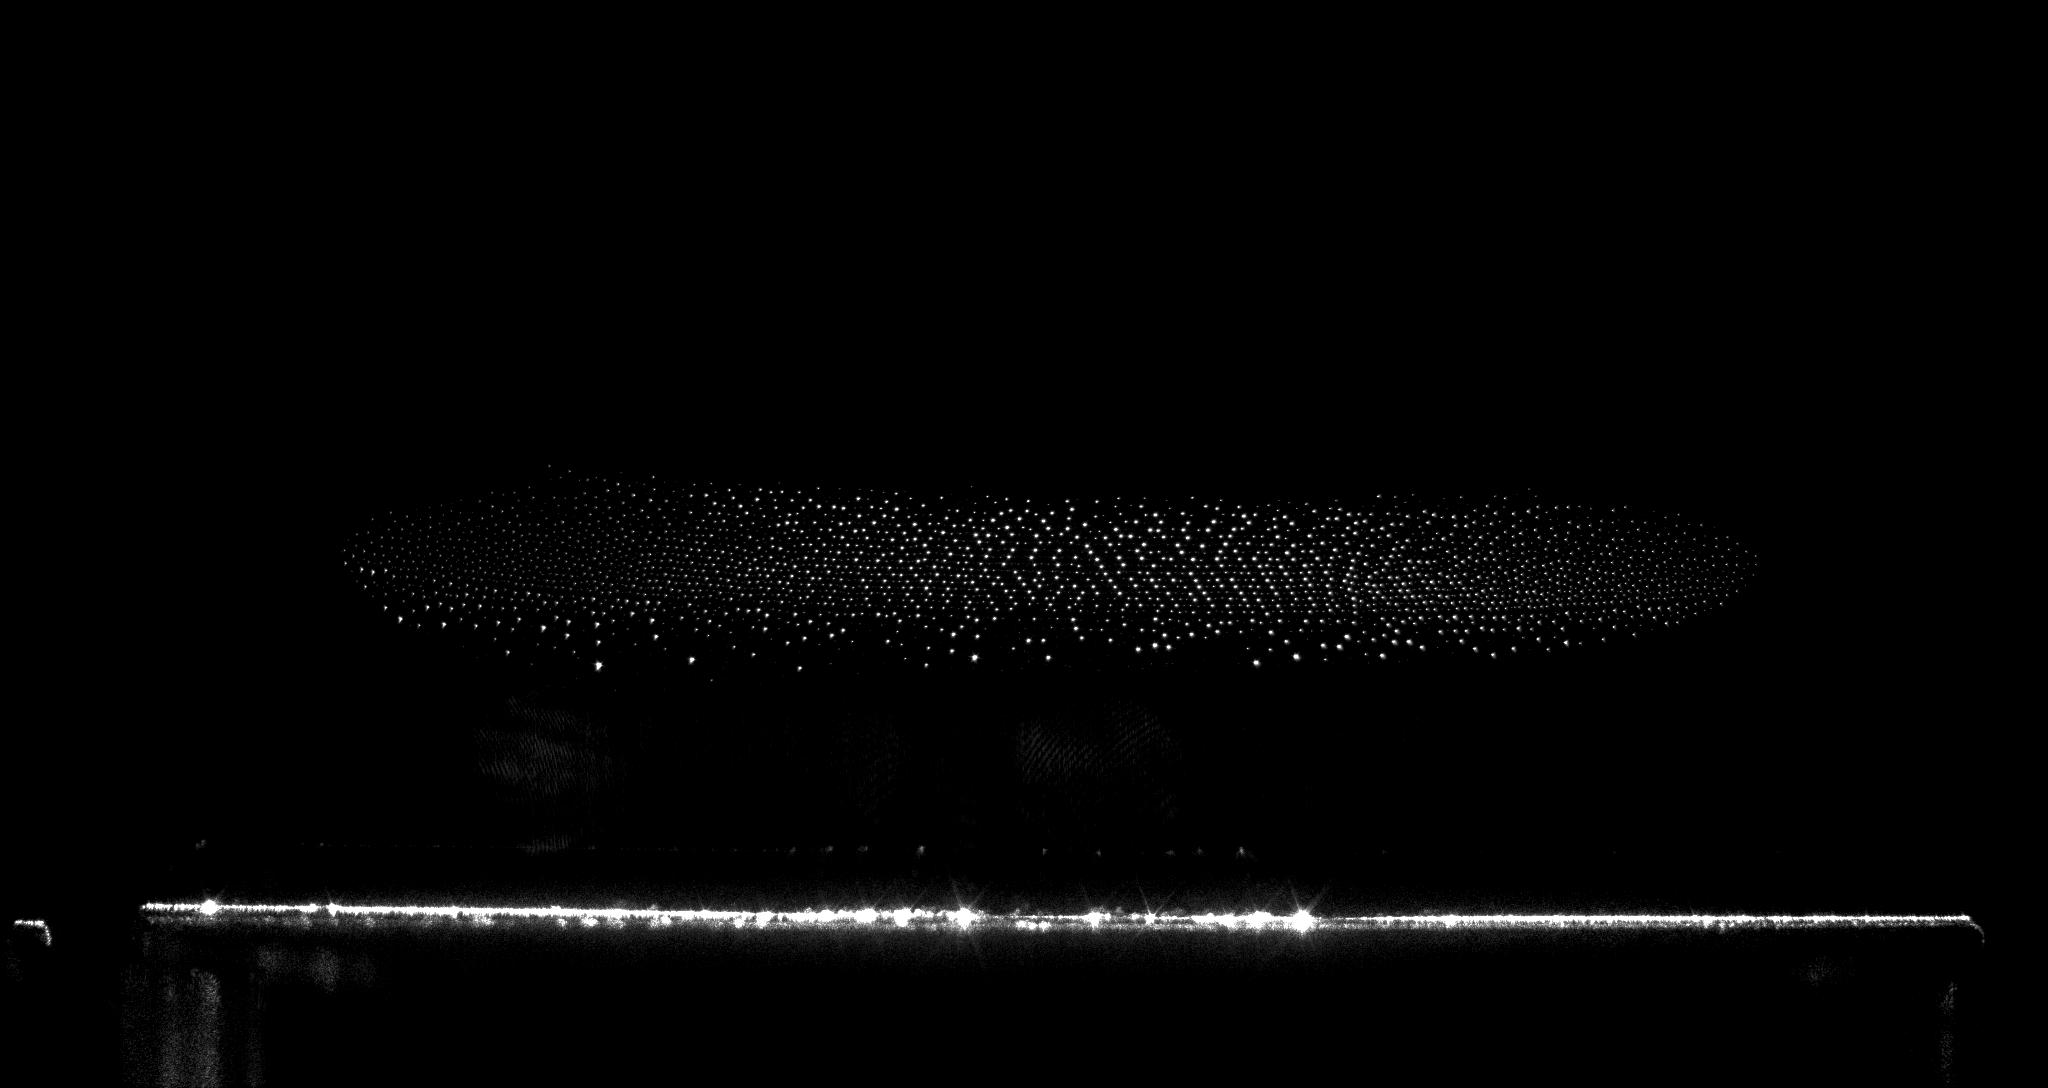
\includegraphics[scale=0.208]{data/Groesse-Teilchenwolke.jpg}
    \caption{Plasmakristall}
    \label{fig:groWo}
\end{figure}

%2. Dimensionen des Kristalls (vorzugsweise in μm) bestimmen:
%a) Gitterabstand in horizontaler (x) und vertikaler (y) Richtung (Messung an mehreren Stellen: Mitte unten, Mitte halbe Höhe, halber Radius unten, halber Radius halbe Höhe. Wenn möglich messen und mitteln Sie über einige (ca. 4-6) Teilchenabstände.),
%b) Breite und Höhe der Teilchenwolke (approximieren Sie den Schnitt durch die Teilchenwolke durch ein sinnvoll gewähltes Rechteck),
%c) Gesamtteilchenzahl (verwenden Sie dazu die von Ihnen gemessenen Teilchenabstände in x und y unter der vereinfachenden Annahme einer kubischen Einheitszelle. Sie können anneh- men, dass z = x und dass Sie den mittleren Schnitt durch die zylindersymmetrische Teilchenwolke sehen). Lassen Sie Ihre Werte vor Ort vom Betreuer prüfen!

\section{Vermessung des Kristalls}
Die Tabellen (\ref{tab:mess-anz} und \ref{tab:anz}) der genauen Messwerte befinden sich im Anhang auf Seite \pageref{tab:mess-anz}. Nachfolgend stehen gerundete Werte; gerechnet wurde mit möglichst genauen.
\subsection{Gitterabstand}
Der ermessene gemittelte horizontale Gitterabstand beträgt $\sim8\,$ Pixel $\approx\,0,19\,$mm. In vertikaler Ausrichtung maßen wir $\sim6\,$Pixel $\approx\,0,15\,$mm.  
\subsection{Ausmaße}
Außmessen ergab eine Breite von $\sim1410\,\text{Pixel}\approx32,4\,mm$ und eine Höhe von $\sim120\,\text{Pixel}\approx2,8\,mm$ des Kristalls. Nebeneinander existieren also $\sim170$ Teilchen: übereinander $\sim20$. 
\subsection{Teilchenanzahl}
Aus obenstehenden Angaben lässt sich unter der Prämisse der rotationssymmetrischen Gleichverteilung und Zylinderartigkeit des Kristalls, die Anzahl der Teilchen in der Wolke bestimmen: $$\bigg(\frac{\text{horizontale Anzahl}}{2}\bigg)^2\cdot\pi\cdot\text{vertikale Anzahl} \approx 425\,000$$



%3. Hausaufgabe: Abschätzung der Partikelladung Q (bei Vernachlässigung der Teilchendichte n d , Angabe bitte in Coulomb und Elementarladungen), des elektrischen Felds E zur Levitation der Partikel, der Debye-Länge λ D , des Coulomb-Kopplungsparameters Γ und des effektiven Parameters Γ eff . (Tipp: Verwenden Sie die Formeln aus der Anleitung. Beachten Sie, dass diese zum Teil in cgs-Einheiten notiert sind!) Sind die Werte plausibel? Kommentieren Sie! Angaben: Teilchenradius a = 1, 0 μm, kT e = 3 eV, kT i = 0, 03 eV, Dichte von Melamin- Formaldehyd 1510 kg/m 3 , F n = F i = F th = 0, T d = 300 K, n i = 10 9 cm −3 .

Mit den folgenden Werten (\cite{1},\cite{TR}) sollen weitere Abschätzungen gemacht werden.

\begin{align}
\text{Partikelradius: }a &= 1\,\mu m \notag\\
\text{Ionentemperatur: }k_BT_i &= 0, 03\,eV\notag\\
\text{Elektronentemperatur: }k_BT_e &= 3\,eV\notag\\
\text{Dichte von Melamin-Formaldehyd: }\rho &= 1510\,\frac{\text{kg}}{\text{m}^3}\notag\\
\text{kinetische Partikeltemperatur: }T_d &= 300\,\text{K}\notag\\
\text{Materialkonstante B: }B&=0,73\notag\\
\text{Dichte der Ionen: }n_i &= 10^9\,\frac{1}{\text{cm}^3}\notag\\
\text{Masse Argon: }M_{Ar}&=39,95\,u\notag\\
\text{F}_n = \text{F}_i = \text{F}_{th} &= 0\notag\\
\text{Erdbeschleunigung: }g&=9,81\,\frac{m}{s^2}\notag\\
\text{Elektronenladung: }e&=1,602\cdot 10^{-19}\,\text{C}\notag\\
\text{Boltzmann-Konstante: }k_B&=1,3807\cdot 10^{-23}\,\frac{J}{K}\notag\\
\text{Dielektrizitätskonstante: }\epsilon_0&=8,85\cdot 10^{-12}\,\frac{As}{Vm}\notag\\
\text{Elektronenmasse: }m_e&=9,11\cdot v10^{-31}\,\text{C}\notag\\
\end{align}


Die Ladung der Partikel Q erhalten wir dann zu:
$$
    Q=Z\cdot e=B\frac{4\pi\epsilon_0ak_BT_e}{e}ln\Big( \sqrt{\frac{T_em_e}{T_iM_{Ar}}}\Big)=-4,97\cdot 10^3\,e=-7,96\cdot 10^{-16}C
$$
  
Um diese Partikel in Schwebe zu halten wird folgende Feldstärke benötigt (Die Plastikkugeln werden als perfekte Kugeln angenähert):
$$
    E=\frac{F}{Q}=\frac{M\cdot g}{Q}=\frac{\rho \frac{4}{3}\pi a^3\cdot g}{Q}=-77,92\,\frac{V}{m}
$$

Die Debye-Wellenlänge ergibt sich zu:
$$
    \lambda_D=\sqrt{\frac{\epsilon_0k_BT_i}{e^2n_i}}=40,7\mu m
$$

Um den Coulomb-Kopplungsparameter $\Gamma$ zu bestimmen benötigen wir zuerst den Partikelabstand\footnote{Diesen mitteln wir aus horizontalem und vertikalen Abständen um eine Richtungsabhängigkeit des Parameters zu vermeiden.} $\Delta$:
$$
    \Delta=\frac{\tilde{x}+\tilde{y}}{2}\approx170\,\mu m
$$

$$
    \Rightarrow\Gamma=\frac{Q^2}{4\pi\epsilon_0\Delta k_BT_d}\approx 8093
$$

Der effektive Coulomb-Kopplungsparameter berücksichtigt zusätzlich die Debye Wellenlänge und den Partikelabstand:
$$
    \Gamma_{eff}=\Gamma\cdot exp\Big(-\frac{\Delta}{\lambda_D}\Big)\approx124
$$ 
Wir haben also mit ein stark gekoppeltes Plasma vorliegen ($\Gamma>1$).

\section{Laserscan}

\begin{figure}[ht]
    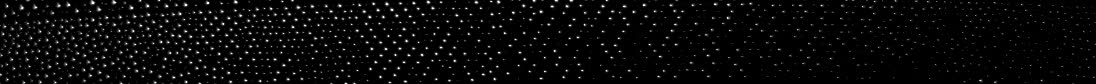
\includegraphics[width=\textwidth]{data/Video0001.jpg}
    \caption{Bildausschnitt des Laserscans}
    \label{fig:videobildausschnitt}
\end{figure}
\begin{figure}[ht]
    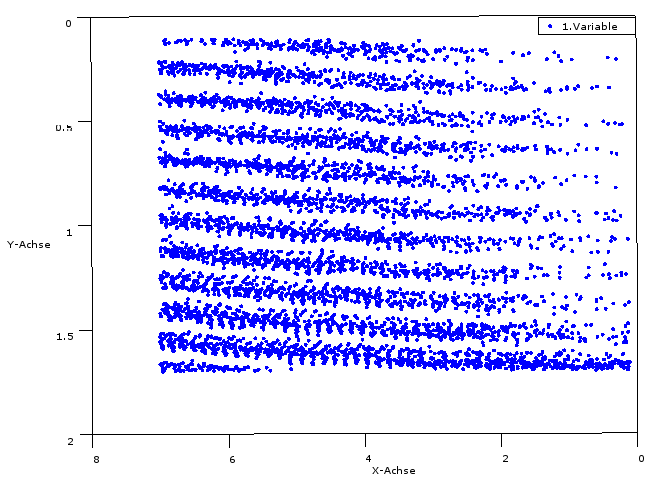
\includegraphics[width=\textwidth]{data/dreiDmodell.PNG}
    \caption{Ergebnis des Laserscans}
    \label{fig:scanerg}
\end{figure}

Nach Wahl eines geigneten Bildausschnitts (siehe Abbilddung \ref{fig:videobildausschnitt}) wird ein Laserscan durchgeführt. Die Ergebnisse des Scans sind in zwei der resultierenden drei Dimensionen in Abb. \ref{fig:scanerg} dargestellt. Die Abstände der Teilchen haben wir ebenfalls bestimmt, das zugehörige Histogramm ist in Abbildung \ref{fig:Abstand} zu finden.

\begin{figure}[ht]
    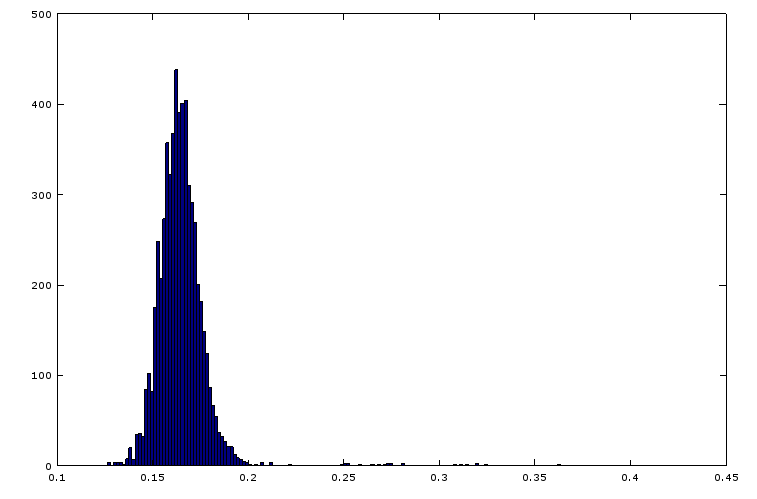
\includegraphics[width=\textwidth]{data/histogramm.PNG}
    \caption{Histogramm der Teilchenabstände}
    \label{fig:Abstand}
\end{figure}

Die Verteilung der Abstände ist recht scharft auf einen Bereich zwischen 0,15-0,18mm begrenzt. Für einen idealen Kristall sollten sich $\delta$-Peaks ergeben. Die Paarkorrelationsfunktion g kann in Abbildung \ref{fig:gr} gesehen werden: Die Fernordnung der Struktur ist dort deutlich zu erkennen.

\begin{figure}[ht]
    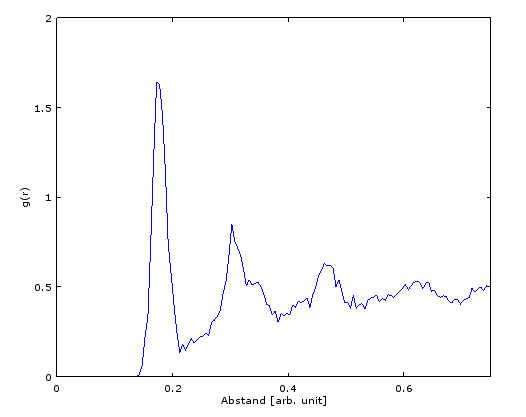
\includegraphics[width=\textwidth]{data/g(r).PNG}
    \caption{Paarkorrelationsfunktion des Kristalls}
    \label{fig:gr}
\end{figure}


\section{Bestimmung des vorliegenden Gittertypes}

Wir betrachten hauptsächlich kubisch\,-\,flächenzentrierte (FCC), kubisch-raumzentrierte (BCC) und hexagonale (HCP) Gitter. Für alle diese Gittertypen wird nun die Paarkorrelationsfunktion g, sowie der Teilchenabstand berechnet. Sämtliche Abbildungen befinden sich auf Seiten \pageref{fig:bccxy}-\pageref{fig:hcpg} im Anhang.
\\
Zur Bestimmung welche Kristallstruktur vorliegt, werden die Bond-Order-Parameter q4 und q6 der idealen Strukturen berechnet und mit den experimentell erhaltenen verglichen. Die berechneten, idealen Parameter sind in Tabelle \ref{tab:bondorder} gegeben.

\begin{table}[ht]
    \centering
    \begin{tabular}{c|ccc}
         & BCC & FCC & HCP \\\hline
         q4 &  0.509 & 0.191 & 0.097\\
         q6 &  0.629 & 0.575 & 0.485\\
    \end{tabular}
    \caption{Bond-Order-Parameter der idealen Strukturen}
    \label{tab:bondorder}
\end{table}

Die Bond-Order Parameter unseres Kristalls werden nun bezüglich ihrer Häufigkeit geplottet: Rot steht für häufig, blau für selten auftretende Werte. Die Abbildungen können in \ref{fig:08} und \ref{fig:12} gefunden werden. Es werden hierfür einmal die 8- und einmal die 12-nächsten Nachbarn betrachtet.

\begin{figure}[ht]
    \centering
    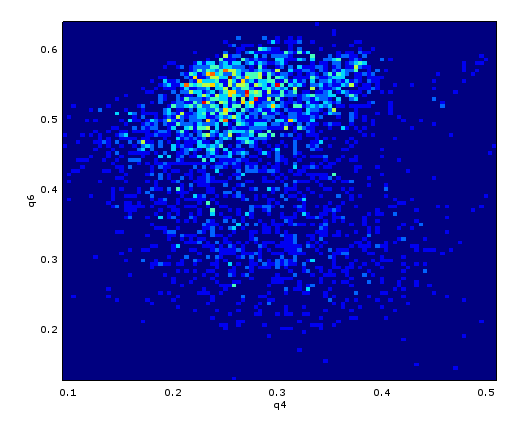
\includegraphics[scale=0.75]{data/rotationinvarianz08.PNG}
    \caption{Bond-Order-Parameter; 8 Nachbarn}
    \label{fig:08}
\end{figure}

\begin{figure}[ht]
    \centering
    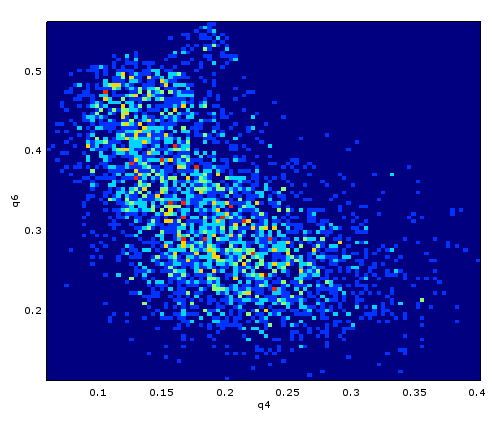
\includegraphics[scale=0.75]{data/rotationinvarianz12.PNG}
    \caption{Bond-Order-Parameter; 12 Nachbarn}
    \label{fig:12}
\end{figure}

In Abbildung \ref{fig:08} lässt sich ein Maximum bei etwa [q4=0,25; q6=0,55] erkennen. Dieser Bereich lässt sich keiner der gegeben Strukturen zuordnen. Dafür wird das Ergebniss beim betrachten der 12-nächsten Nachbarn in Abbildung \ref{fig:12} deutlicher: Es lassen sich eindeutig Bereiche der HCP-Struktur zuordnen, außerdem ist eine kleine Domäne der FCC-Struktur zu finden (vgl. mit Tabelle \ref{tab:bondorder}). BCC-Domänen liegen hingegen nicht vor.

\section{Grenzbereiche}
Abschließend soll die Struktur der Plastikteilchen bei Änderungen der Spannung und des Druckes untersucht werden. Als Ausgagssrtuktur wird ein Druck von 40\,Pa und eine RF-Spannung von 0,15\,eV verwendet (siehe als Vergleich Bild \ref{fig:groWo}).

\subsection{Änderung des Druckes}
Wir verringern nun den Druck von 40\,Pa auf 14\,Pa. Ab 32\,Pa beginnen die Partikel des Kristalls in den unteren Schichten zu oszillieren, ab 24\,Pa ist die Struktur nicht mehr zu erkennen; Der Kristall ist \glqq geschmolzen\grqq{}. Durch Verringerung des Druckes wird die Partikelladung der Teilchen und damit der Parameter $\Gamma$ kleiner. Zudem verringert sich die Reibung der Partikel an den Gasatomen, wodurch die kinetische Energie der Partikel weiter erhöht wird. Dadurch wird die Kristallstruktur aufgebrochen.

\begin{figure}[ht]
    \centering
    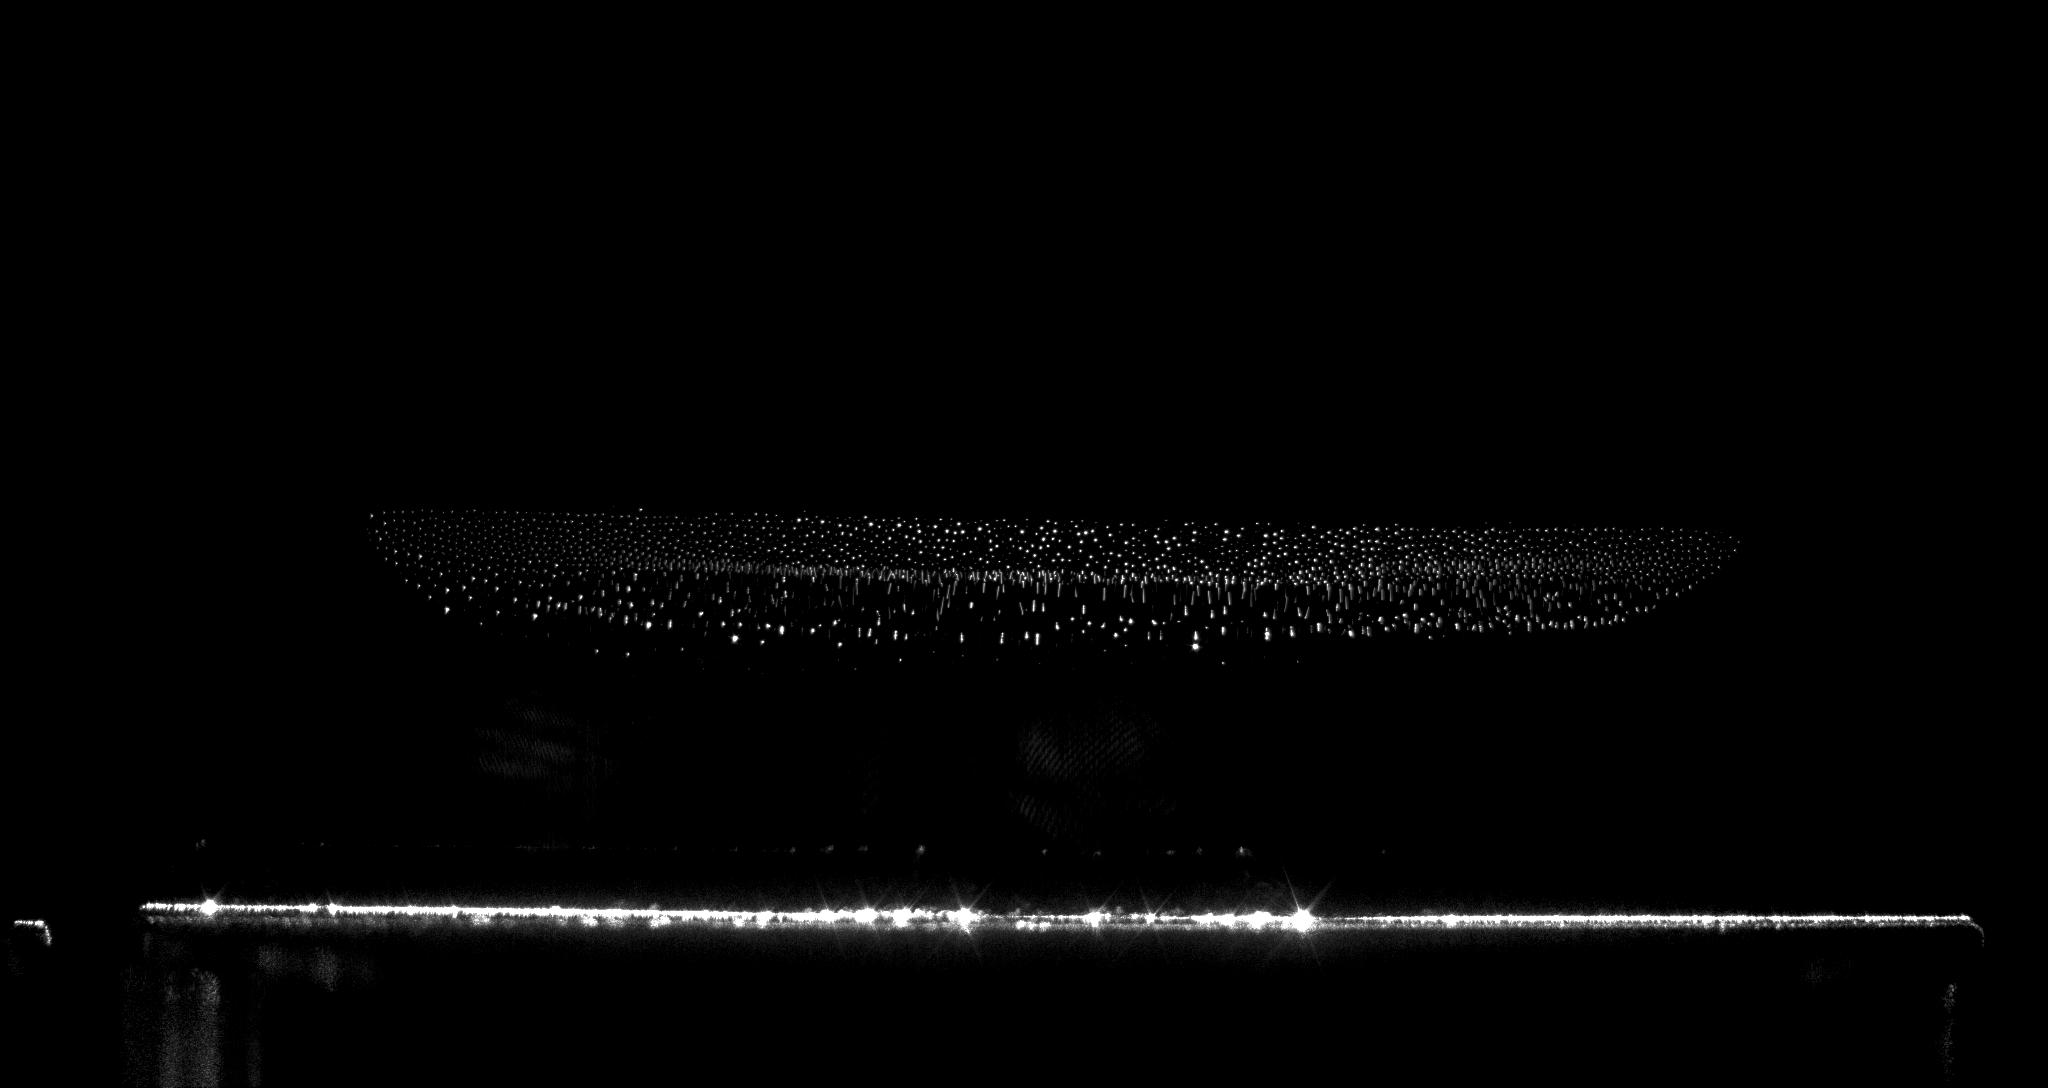
\includegraphics[width=\textwidth]{data/32pa.jpg}
    \caption{Partikelwolke bei 32\,Pa}
    \label{fig:32pa}
\end{figure}

\begin{figure}[ht]
    \centering
    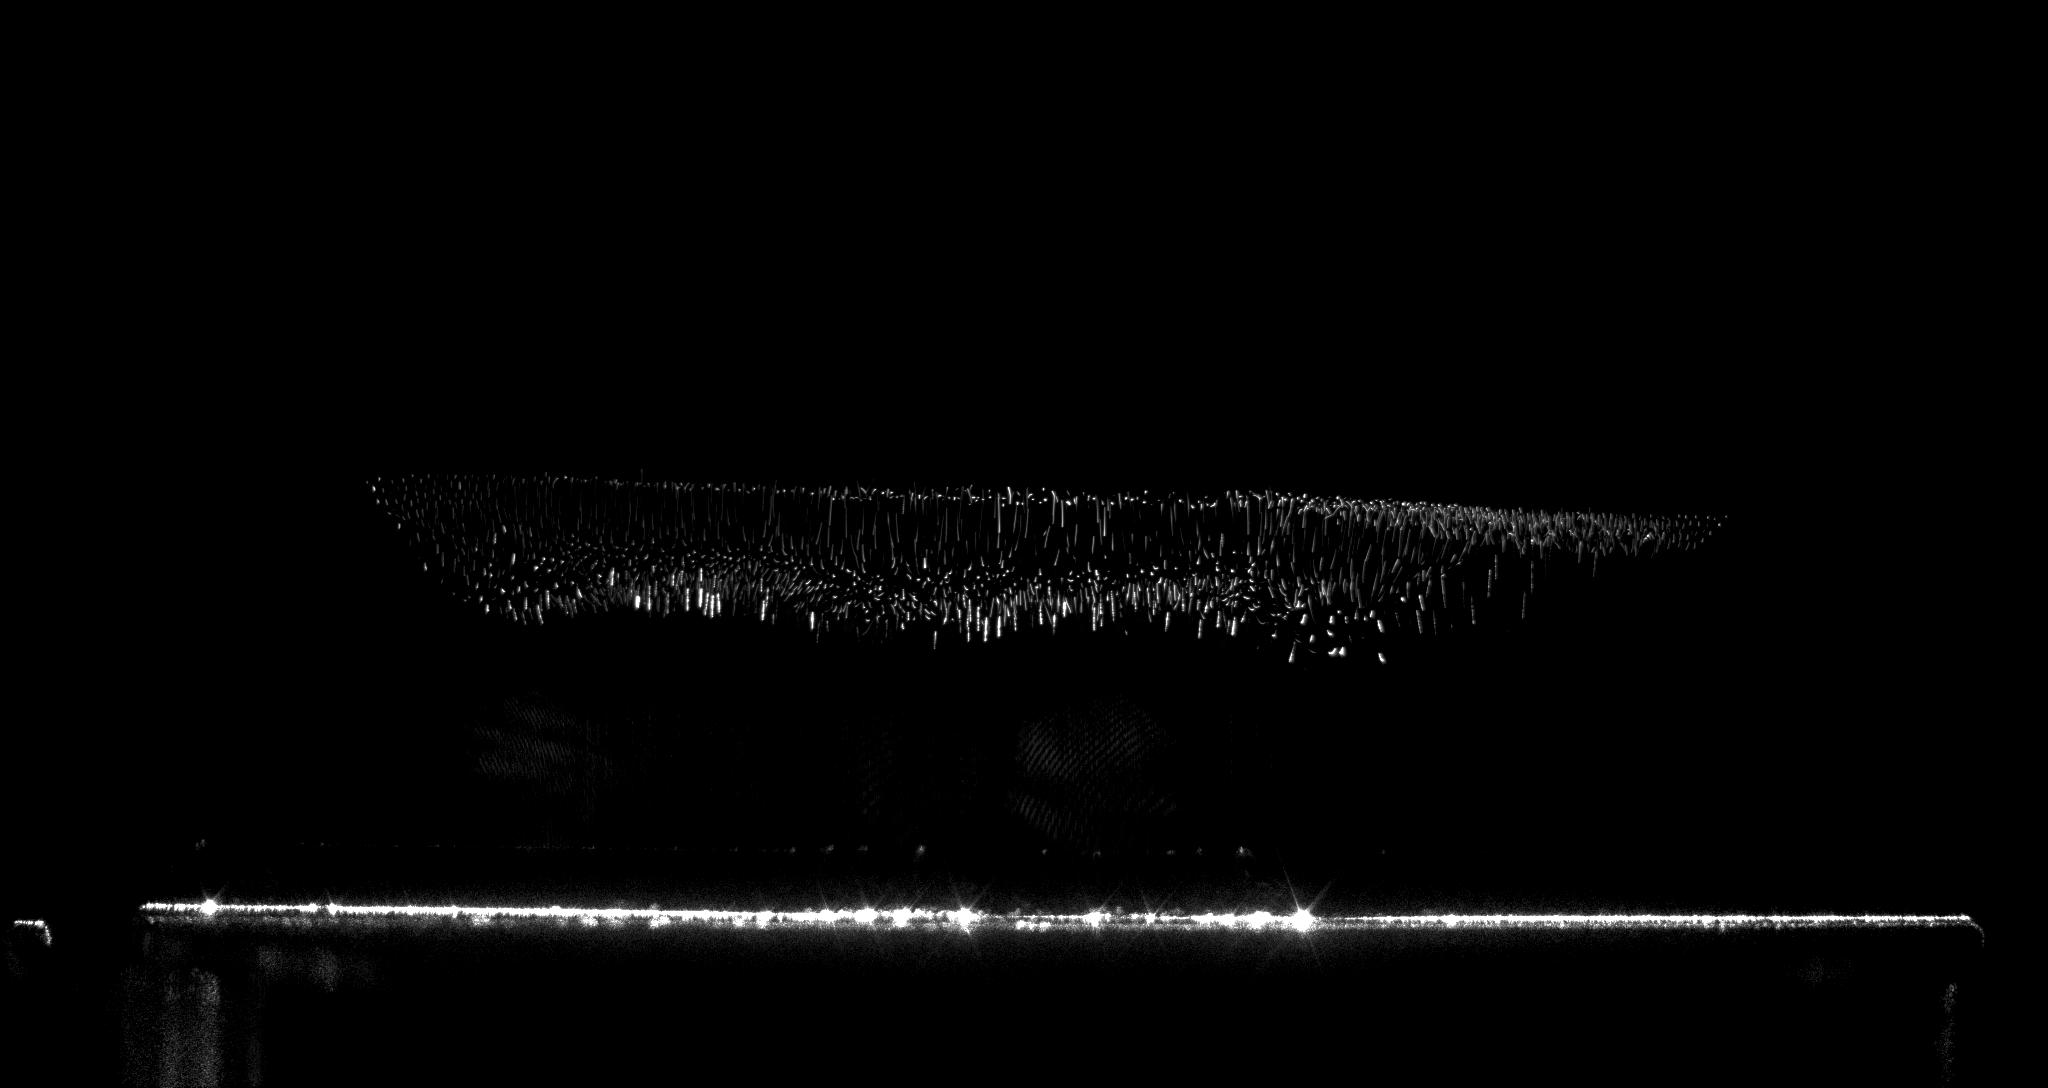
\includegraphics[width=\textwidth]{data/24pa.jpg}
    \caption{Partikelwolke bei 24\,Pa}
    \label{fig:24pa}
\end{figure}

\subsection{Änderung der Spannung}
Bei 40\,Pa erhöhen wir nun die Spannung von 0,15\,V auf 1,5\,V. Der Kristall wird dabei vertikal zusammengedrückt und horizontal gestreckt. Hierbei ändern sich die Teilchenabstände in vertikaler Richtung von etwa 6,25 zu 6 Pixeln, in horizontaler Richtung bleibt der Teilchenabstand konstant.

\begin{figure}[ht]
    \centering
    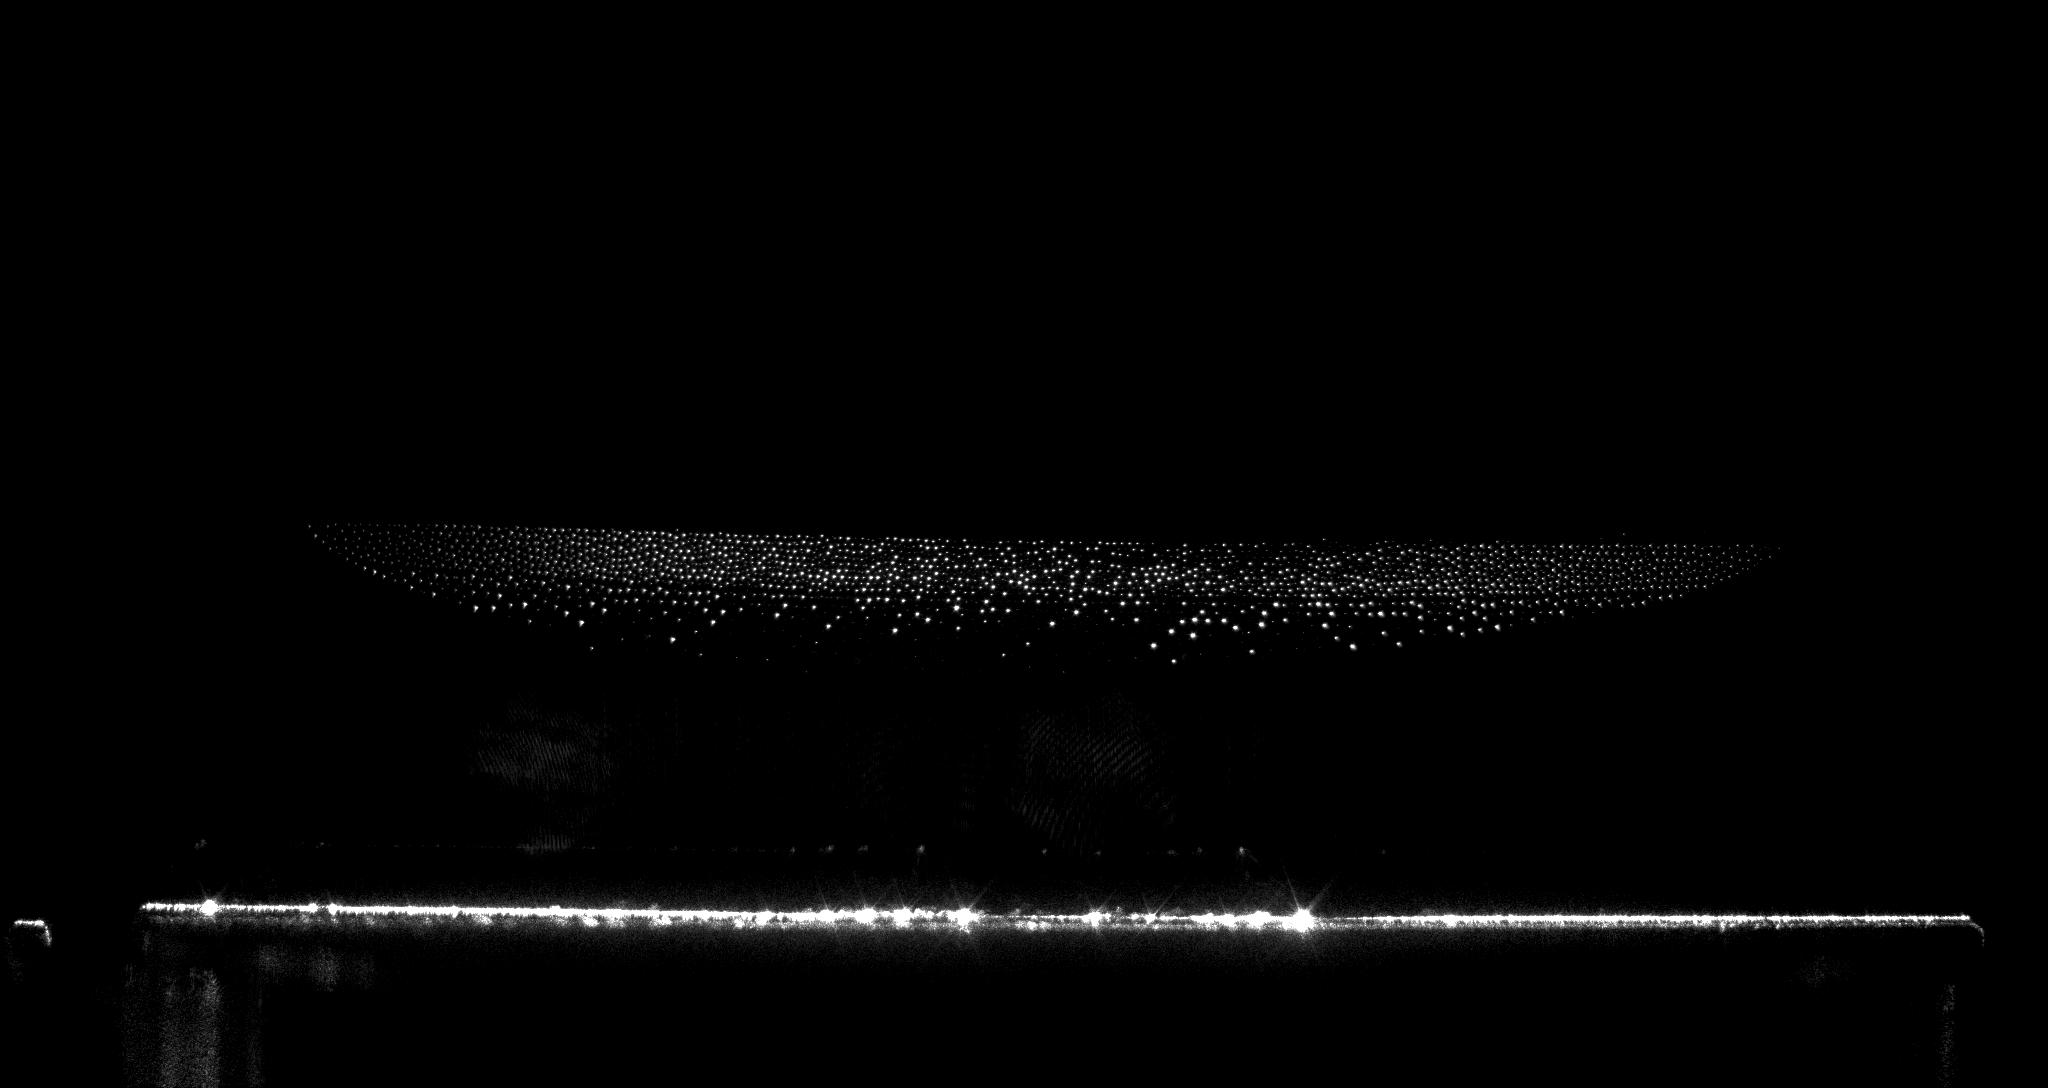
\includegraphics[width=\textwidth]{data/0,15V.jpg}
    \caption{Partikelwolke bei 0,15\,V}
    \label{fig:015v}
\end{figure}

\begin{figure}[ht]
    \centering
    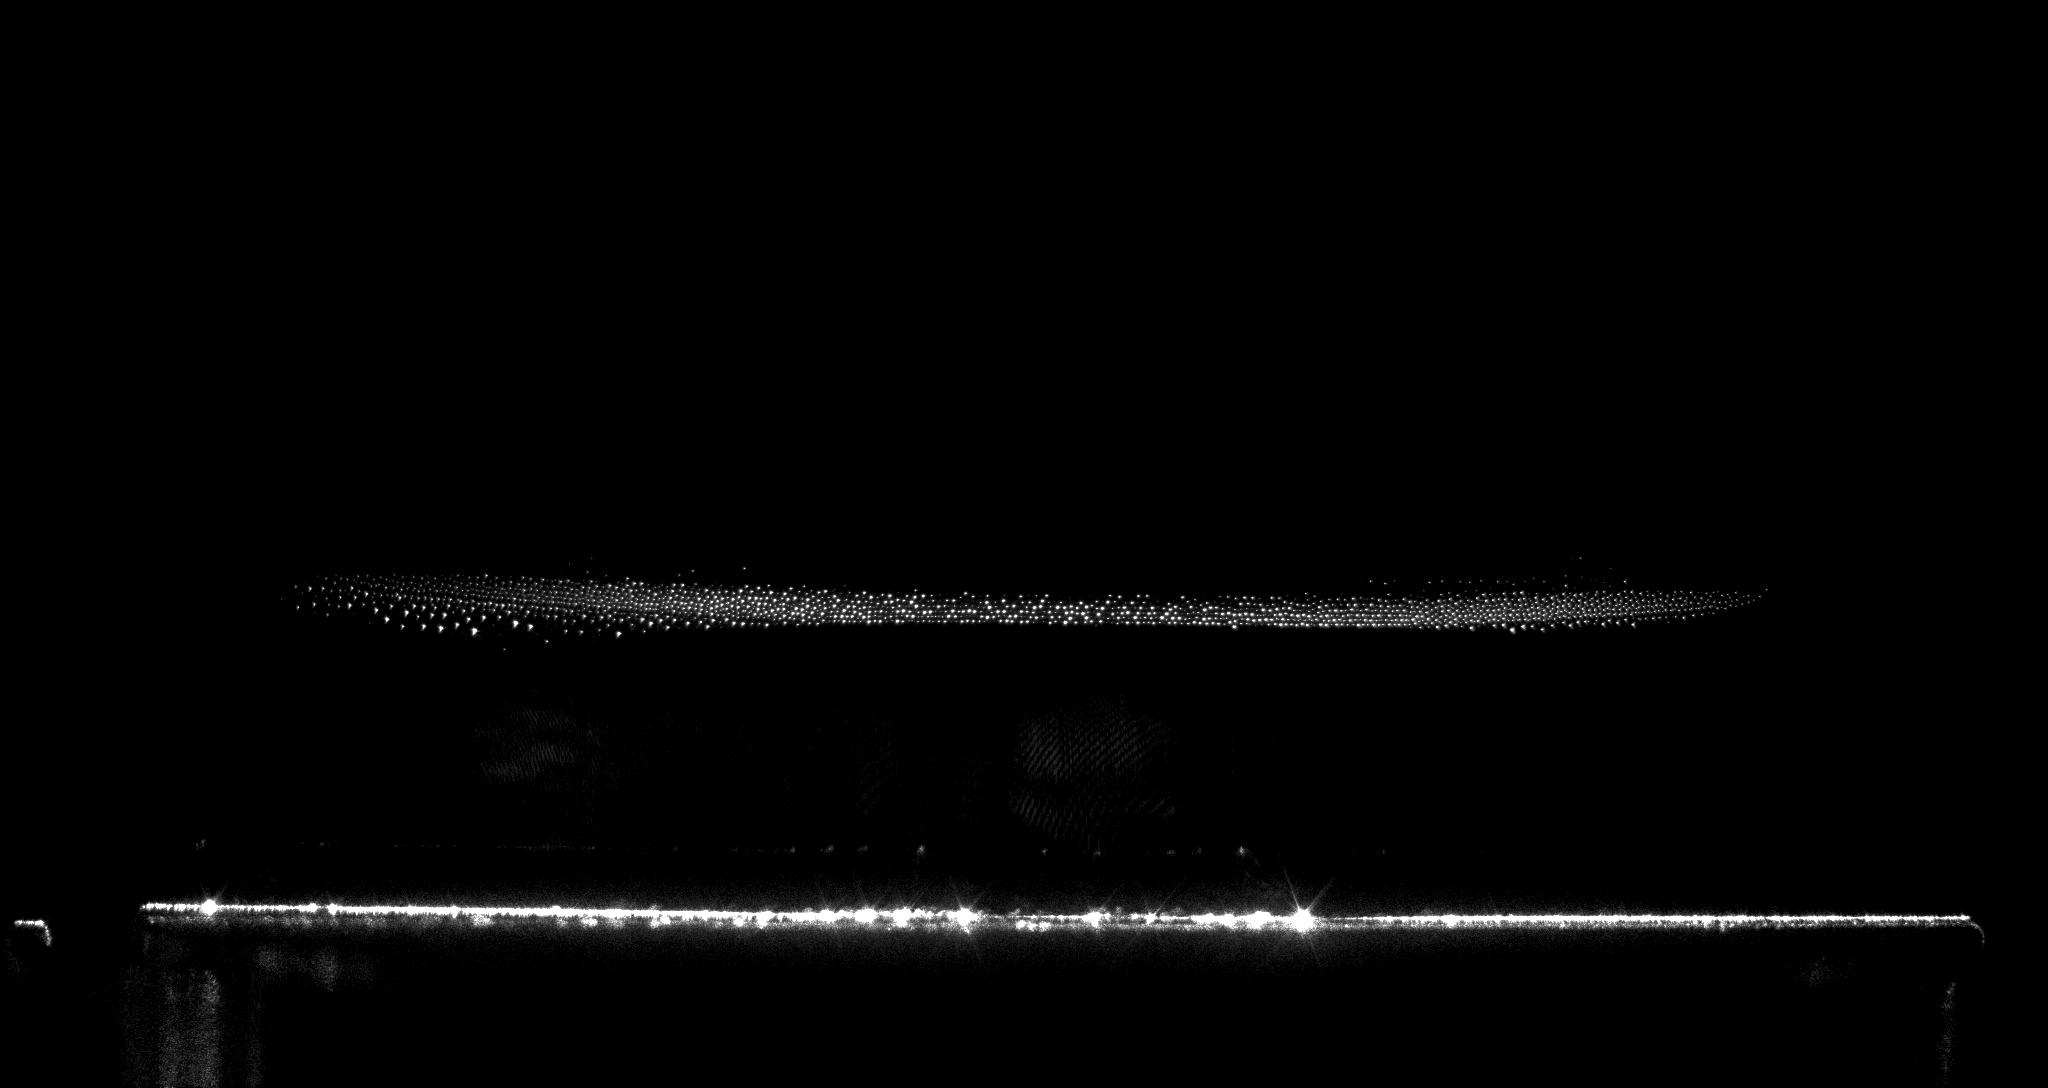
\includegraphics[width=\textwidth]{data/1,5V.jpg}
    \caption{Partikelwolke bei 1,5\,V}
    \label{fig:15v}
\end{figure}

Schlußendlich wird die Spannung in 0,01\,V Schritten heruntergefahren: Der Kristall erlangt zunächst wieder seine ursprünglichen Ausdehnungen. Bei einer Spannung von 0,11\,V ist das elektrische Feld nicht mehr stark genug um das Plasma zu erhalten und die Partikel stürzen aufgrund der Erdbeschleunigung abrupt herab.

\chapter{Fazit}
Alle theoretischen Überlegungen in der Vorbereitung sind mit unseren Messungen bestätigt. Der Versuch ist ein interessante Möglichkeit ein aktuelles Forschungsthema kennenzulernen und wurde erfolgreich durchgeführt.